\chapter{Cálculo de cargas}


\section{Superfícies Aerodinâmicas}

Para o dimensionamento das estruturas e componentes da aeronave é necessário determinar qual a ordem de grandeza dos esforços a que estarão submetidos durante a operação da aeronave. As condições consideradas para determinação das cargas estáticas foram a velocidade de mergulho, em fator de carga máximo, ou seja, as condições mais extremas do diagrama V x n. Cargas inerciais foram mais uma vez desconsideradas, aplicando-se assim uma abordagem conservadora ao não levar em conta peso da asa e do motor.
As condições de trimagem foram corrigidas em relação ao cálculo preliminar de cargas e o novo valor de ângulo de ataque de asa utilizado foi de aproximadamente 1,15°.
Os valores encontrados para as cargas são mostrados nas \autoref{fig:cort_ASA} a \autoref{fig:torc_EV}

\begin{figure}
\centering
    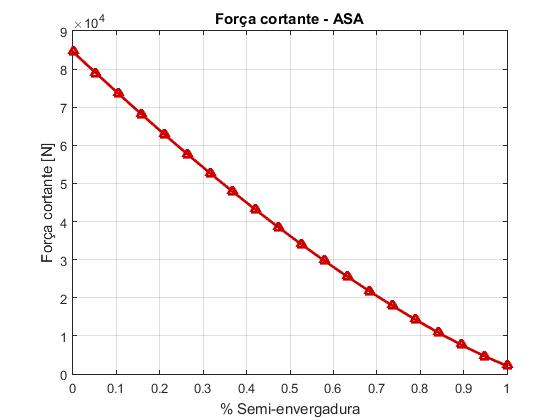
\includegraphics[width=\textwidth]{cargas/imagens/cort_ASA.jpg}
\caption{Força cortante distribuída em uma semi-asa}
\label{fig:cort_ASA}
\end{figure}

\begin{figure}
\centering
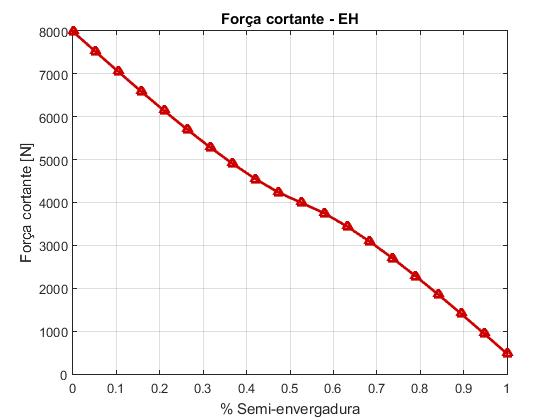
\includegraphics[width=\textwidth]{cargas/imagens/cort_EH.jpg}
\caption{Força cortante distribuída na semi-envergadura da empenagem horizontal}
\label{fig:cort_EH}
\end{figure}

\begin{figure}
\centering
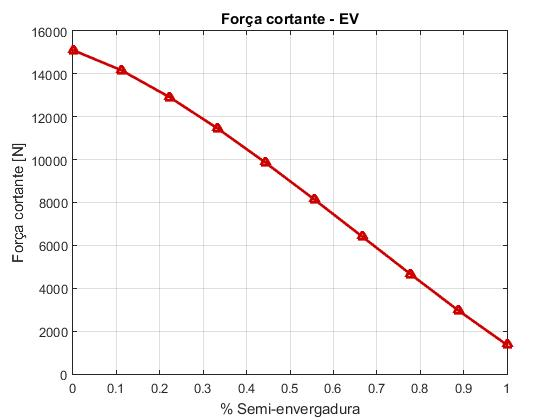
\includegraphics[width=\textwidth]{cargas/imagens/cort_EV.jpg}
\caption{Força cortante distribuída na empenagem vertical}
\label{fig:cort_EV}
\end{figure}

\begin{figure}
\centering
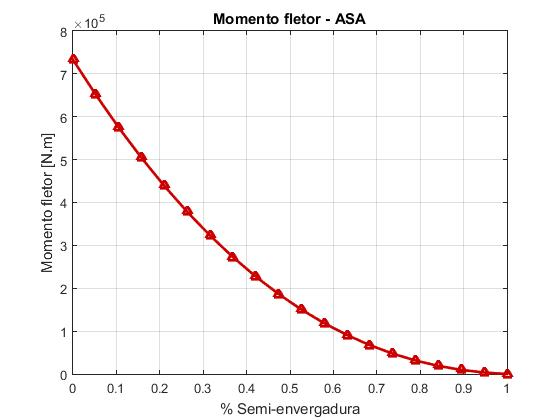
\includegraphics[width=\textwidth]{cargas/imagens/flet_ASA.jpg}
\caption{Momento fletor distribuído em uma semi-asa}
\label{fig:flet_ASA}
\end{figure}

\begin{figure}
\centering
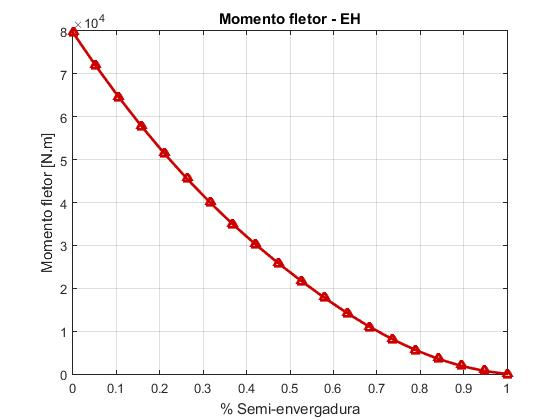
\includegraphics[width=\textwidth]{cargas/imagens/flet_EH.jpg}
\caption{Momento fletor distribuído na semi-envergadura da empenagem horizontal}
\label{fig:flet_EH}
\end{figure}

\begin{figure}
\centering
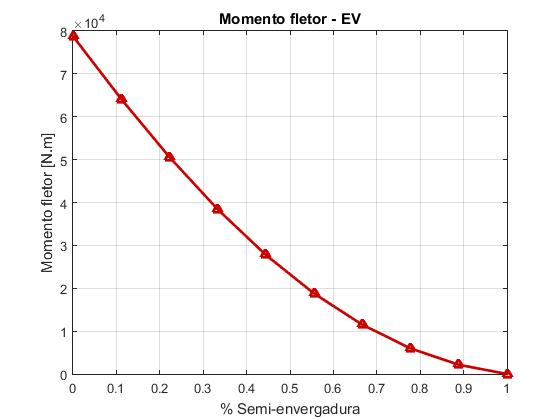
\includegraphics[width=\textwidth]{cargas/imagens/flet_EV.jpg}
\caption{Momento fletor distribuído na empenagem vertical}
\label{fig:flet_EV}
\end{figure}

\begin{figure}
\centering
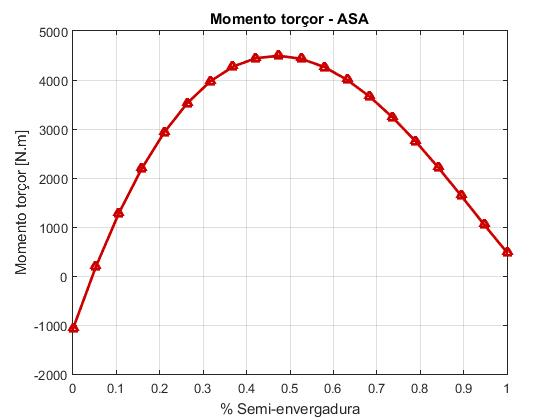
\includegraphics[width=\textwidth]{cargas/imagens/torc_ASA.jpg}
\caption{Momento torçor distribuído em uma semi-asa}
\label{fig:torc_ASA}
\end{figure}

\begin{figure}
\centering
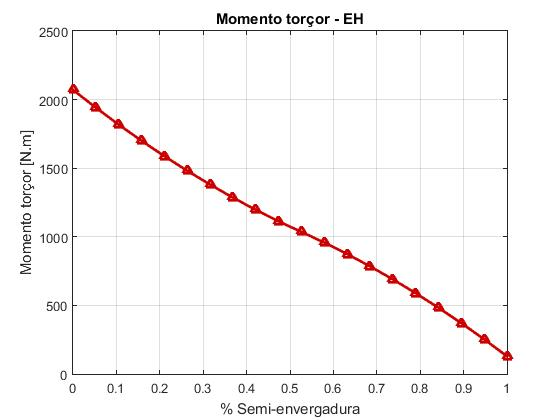
\includegraphics[width=\textwidth]{cargas/imagens/torc_EH.jpg}
\caption{Momento torçor distribuído na semi-envergadura da empenagem horizontal}
\label{fig:torc_EH}
\end{figure}

\begin{figure}
\centering
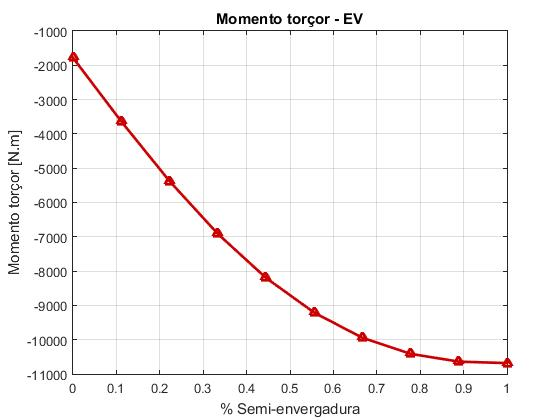
\includegraphics[width=\textwidth]{cargas/imagens/torc_EV.jpg}
\caption{Momento torçor distribuído na empenagem vertical}
\label{fig:torc_EV}
\end{figure}


\section{Trem de Pouso}

Foram também calculadas as cargas no trem de pouso para diferentes condições recorrentes na operação da aeronave. São elas: pouso em três rodas, pouso em duas rodas e pouso em uma única roda. No segundo e terceiro casos, são considerados apenas os trens de pouso principais. Em todas as três situações, entretanto, consideram-se três sub-casos: pouso alinhado, ou seja, com o eixo longitudinal da aeronave apontado na direção de deslocamento, pouso não alinhado com as rodas em aceleração (ou seja, com velocidade tangencial nula), e pouso não alinhado com as rodas em velocidade tangencial igual à velocidade de deslocamento da aeronave. Todos estes casos são exigidos de acordo com a CFR Part 23.
Os resultados para os cálculos de cargas em trem de pouso são mostrados na \autoref{fig:cargas_tdp}.

\begin{figure}
\centering
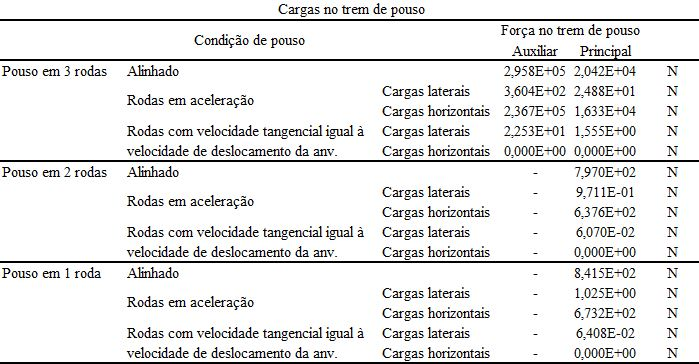
\includegraphics[width=\textwidth]{cargas/imagens/Cargas_tdp.jpg}
\caption{Cargas no trem de pouso}
\label{fig:cargas_tdp}
\end{figure}
